\label{sec:unittests_future}
Unit-tests have been an established part of the programmer's toolkit since it was formalized in 1986\cite{1986ansi} and continue to be a great resource for assuring that builds are working correctly between changes. Another use that has been identified is obviously to ensure that submitted code meets some requirements by giving input to pre-specified functions and checking that the functions act correctly.

One could imagine an extension to tester that would enable teachers to upload unit tests and run them against the supplied code. This could be done by supplying an additional step akin to the compilation step already implemented in the runner and adding the framework as a dependency in the docker image creation. However, with the way that the test-runner is currently implemented, care must be taken to avoid letting the tested code edit or read the unit tests.
\begin{figure}[hb]
    \centering
    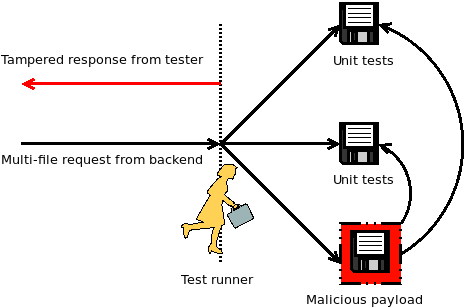
\includegraphics[width=.5\linewidth]{img/unittest_editing.png}\label{fig:unit_tamper}
    \caption{An adversary could use their program to tamper with or dump unit-tests.}
\end{figure}

Since not every interpreter nor runtime makes it easy to run programs that are not on disk (for instance, a build of python tested during development expected its scripts to end with \texttt{.py} to at all be valid, whereas the line-feed reader expected input to be semi-colon separated), it saves the file to disk and runs the programs on it. In addition, from what cursory studies revealed, few unit testing suites provide support for multi-file tests to be read from \texttt{stdin} without any hassle. Thus, it can't be assumed that it is a task that teachers would be confident with doing, which motivates saving all files to disk before testing. But, since the files are stored on disk, the previously mentioned exploit needs to be mitigated, possibly through tricks similar to those used in section~\ref{sec:dumping}.
%tester was built under the assumption that it would only test one file at a time and 
